\documentclass[a4paper, 12pt]{article}
%\documentclass{book}

% Important Packages:
 \usepackage{amsmath}    % need for subequations
 \usepackage{amsfonts}
 \usepackage{amsthm}
 \usepackage{graphicx}   % need for figures
 \usepackage{verbatim}   % useful for program listings
 \usepackage{fancyvrb}
  
 % Useful macros 
 \def\tcb#1{\color{blue}{#1}}
 \def\tcr#1{\color{red}{#1}}	
 \def\tcg#1{\color{green}{#1}}
 \def\be{\begin{eqnarray}}	 	\def\ee{\end{eqnarray}}
 \def\bea{\begin{eqnarray}}	 	\def\eea{\end{eqnarray}}
 \def\bean{\begin{eqnarray*}}	\def\eean{\end{eqnarray*}}
 
 \def\D{\displaystyle}
 \def\T{\textstyle}
 \def\l{\left}
 \def\r{\right}
 \def\nf{n_{\!f}} % quark flavours
 \def\pa{\partial}
 \def\eg{e.\,g.}
 \def\ie{i.\,e.}

 \def\be{\begin{equation}}
 \def\ee{\end{equation}}
 \def\bea{\begin{eqnarray}}
 \def\eea{\end{eqnarray}}
 \def\bean{\begin{eqnarray*}}
 \def\eean{\end{eqnarray*}}
 \def\gsim{\mathrel{\rlap{\lower0.2em\hbox{$\sim$}}\raise0.2em\hbox{$>$}}}
 \def\ksim{\mathrel{\rlap{\lower0.2em\hbox{$\sim$}}\raise0.2em\hbox{$<$}}}
 \def\kg{\mathrel{\rlap{\lower0.25em\hbox{$>$}}\raise0.25em\hbox{$<$}}}
 
 \def\AA{${\buildrel_{\circ} \over {\mathrm{A}}}$}
 \def\bm#1{\mbox{\boldmath$#1$}}
 \newcommand{\eq}[1]{(\ref{#1})} 
 \def\pd{\partial}
 \def\d{\textrm{d}} 
 \def\T{\textstyle}
 \def\eg{e.\,g.}	% exempli gratia (for the sake of example)
 \def\ie{i.\,e.}	% id est (that is)


 % Page configuration:
 \topmargin -2.0cm
 \oddsidemargin -0.85cm
 \evensidemargin -0.85cm
 \textwidth 18cm
 \textheight 24cm
 

\begin{document}

\begin{center}
\textbf{Stellenbosch Camp December 2017 \\ Senior Test 5} \\
\textbf{Solutions}
\end{center}


\begin{enumerate}

    % QUESTION 1
    \item[1.] 
    
    
    % QUESTION 2
    \item[2.] 
    
    
    % QUESTION 3
    \item[3.] Let $O$ be the midpoint of $BC$. As $ABC$ is right-angled, we have $O$ the centre of the circle through $ABC$. Let $N$ be the intersection of $BP$ and $OC'$ and let $M$ be the intersection of $CI$ and $OC'$. Note that $OC'$ is parallel to $AC$ by the midpoint theorem. Hence $\angle OMC = \angle ACM = \angle OCM$ as $CI$ is the angle bisector of $\angle ACB$. Hence, $OM = OC$ which implies $O$ lies of the circumcircle of $ABC$. As $AMCB$ cyclic, we have $\angle AMC = \angle ABC = 45^\circ$.
    
    Note that $\angle AMC' = \angle AMC + \angle CMO = 45^\circ + 22.5^\circ = 67.5^\circ$. Also, $\angle BNC' = 90^\circ - \angle C'BN = 67.5^\circ$. Since $AC' = C'N$ this implies $\triangle AMC'$ and $\triangle BNC'$ congruent, hence $C'$ is the midpoint of $MN$.
    
    The claim that $X$ is the midpoint of $PC$ then follows since $\triangle MIN$ is similar to $\triangle CIP$ and $C'IX$ collinear.
        
    \begin{figure}[h!]
        \centering
        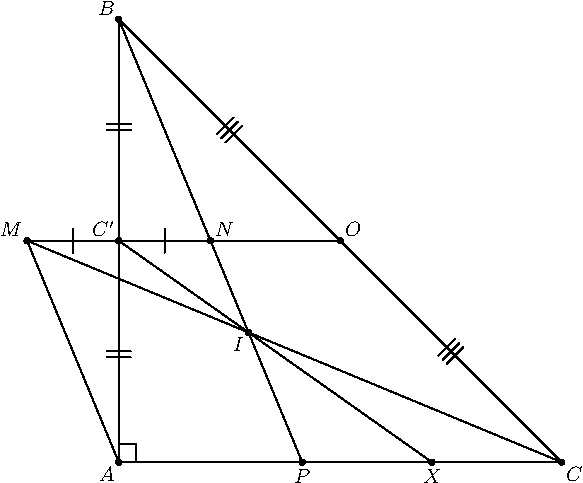
\includegraphics[width=0.4\textwidth]{seniortest5_q3.pdf}
    \end{figure}
    

    % QUESTION 4
    \item[4.] \textit{Austrian Mathematical Olympiad 2011, Final Round, part 2, day 1} \\ Since 3 pins (P) or 2 brackets (B) may not lie in a row, they may not do so on an individual brick. This means that there are only three different types of brick: PBPP (type A); PPBP (type B); BPB (type C). Naming the number of possible patterns of $n$ bricks with a brick of type A at the end $a_n$, and analogously $b_n$ and $c_n$ for types B and C, the number we wish to determine is $s_n=a_n+b_n+c_n$. Due to the restrictions on the bricks, we see that $a_{n+1}=b_n+c_n$, $b_{n+1}=c_n$ and $c_{n+1}=a_n+b_n$ with starting values $a_1=b_1=c_1=1$. This yields:
\begin{equation*}
s_{n+1}=s_n+(b_n+c_n)=s_n+(a_{n-1}+b_{n-1}+c_{n-1})=s_n+s_{n-1}
\end{equation*}
with $s_1=3$ and $s_2=5$. We see that the resulting sequence $s_n$ us simply the Fibonacci sequence starting from the fourth element, and so $s_n=F_{n+3}$.
    
    
    % QUESTION 5
    \item[5.] We first prove that $f$ is injective. Let $a, b \in \mathbb{N}$ such that $f(a) = f(b)$. Letting $w = x = y = 1$ and $z = a$ and $z = b$ for the LHS and RHS respectively, we obtain:
    \begin{align*}
        f(a) = f(b) &\implies f(f(f(a))) f(f(f(a))) =  f(f(f(b))) f(f(f(b))) \\
        &\implies a^2 f(f(1)) f(1) = b^2 f(f(1)) f(1) \\ &\implies a = b
    \end{align*} 
    as $f(f(1)) f(1) \in \mathbb{N}$. Hence $f$ is injective. Setting $z = 1$ and $w = f(f(1))$, we obtain:
    \begin{align*}
        f(f(f(1))) f(f(f(1)) x f(yf(1))) &= f(xf(y)) f(f(f(1))) \\
        \implies \quad f(f(f(1)) x f(yf(1))) &= f(xf(y)) \\
        \implies \qquad f(f(1)) x f(yf(1)) &= x f(y)
    \end{align*}
    where the last line is obtained due to injectivity. We now let $f(1) = c$ and set $x = 1$. The last equation therefore yields:
    $$ f(c) f(yc) = f(y) $$
    For $y = 1$, we get: $f(c) f(c) = f(1) = c$. For $y = c$, we get: $f(c) f(c^2) = f(c)$ which implies $f(c^2) = 1$. For $y = c^2$, we get: $f(c) f(c^3) = f(c^2) = 1$ which implies $f(c) = f(c^3) = 1$ since the only product of two natural numbers which gives 1 is $1 \cdot 1$. By injectivity, we obtain: $c = c^3$, hence $f(1) = c = 1$.
    
    Letting $z = y = 1$ in the original equation now gives us:
    $$ f(wx) = f(x) f(w) $$
    Hence, $f$ is multiplicative, which implies:
    $$ f(n!) = f(1) f(2) f(3) \dots f(n) $$
    As $f$ is injective, each of the factors on the right hand side must be a distinct natural number. Since the product of $n$ distinct natural numbers is at least $n!$, we obtain $f(n!) \geq n!$ which completes the proof.
    
    
    
    % QUESTION 6
    \item[6.] Let $a_n$ be the number on the blackboard after the $n^{th}$ step and let $i_n = a_n - a_{n-1}$ be the increase at the $n^{th}$ step. We claim that for any $n$, either $i_n = 1$ or $a_n = 3n$. We shall prove this by induction.
    
    Note that we have $i_1=i_2=i_3=i_4=1$ and $i_5=5\neq 1$ but $a_5=15$. Hence the base case is proven. Let's assume that for some natural $n$ we have $i_n\neq 1$ and $a_n=3n$. Let $k$ be the least natural number such that $i_{n+k}\neq 1$. Note that
    $$ i_{n+k}=\textrm{gcd}(n+k, i_{n+k-1})=\textrm{gcd}(n+k, 3n+k-1)=\textrm{gcd}(n+k, 2k+1) $$
    
    If $2k+1$ is prime, we hence obtain $i_{n+k}=2k+1$ prime and $a_{n+k}=3n+k-1+2k+1=3(n+k)$. This would prove the induction hypothesis, which would hence solve the problem.
    
    We are now only left to prove $2k+1$ is prime. Assume for contradiction $2k+1$ is not prime. Consider any prime divisor $p|\textrm{gcd}(n+k, 2k+1)$. We have
     $$ p|2k+1, p\neq 2k+1 \quad \Longrightarrow \quad p \leq \frac{2k+1}{3} \quad \Longrightarrow \quad p<k $$
     
     Now consider
     $$ i_{n+k-p}=\textrm{gcd}(n+k-p, 3n+k-p-1)=\textrm{gcd}(n+k-p, 2k+1-2p) $$
     
     Now, since $p|n+k, 2k+1,$ we have $p|\textrm{gcd}(n+k-p, 2k+1-2p)$ which implies $ i_{n+k-p} \neq 1$ contradicting the minimality of $k$.
     
     Hence $2k+1$ is prime, which completes the proof.
    
    
\end{enumerate}


\centering
\begin{BVerbatim}
\end{BVerbatim}

\end{document}

